%\section{Cahn-Hilliard Examples}

%%%%%%%%%%%%%%%%%%%%%%%%%%%%%%%%%%%%%%%%%%%%%%%%%%%%%%%%%%%%%%%%%%%%%
\royslide{Phase Separation}{

\royitemizebegin
\item Random perturbations in initial conditions rapidly segregate
into two distinct phases, divided by a labyrinth of sharp interfaces
\item Rapid anti-diffusionary process
\royitemizeend

\begin{center}
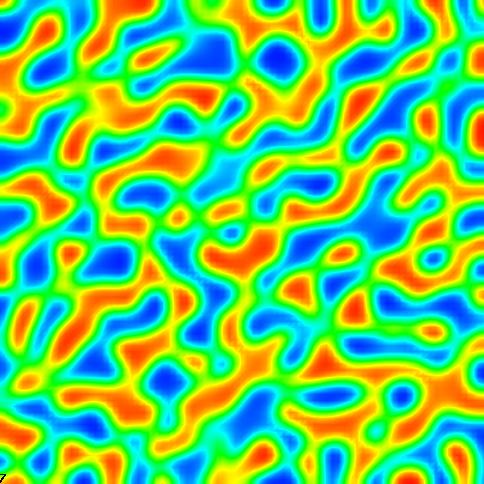
\includegraphics[width=.3\textwidth]{figs/ch010}
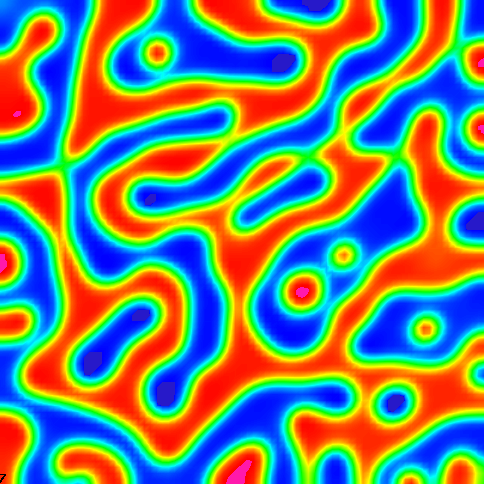
\includegraphics[width=.3\textwidth]{figs/ch050}
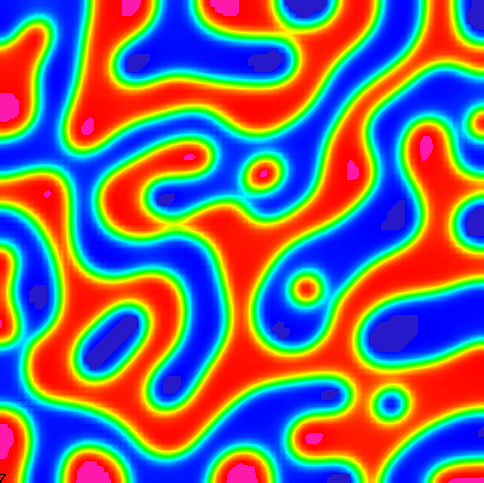
\includegraphics[width=.3\textwidth]{figs/ch100}
\end{center}
}


%%%%%%%%%%%%%%%%%%%%%%%%%%%%%%%%%%%%%%%%%%%%%%%%%%%%%%%%%%%%%%%%%%%%%
\royslide{Spinodal Decomposition}{

\royitemizebegin
\item Over long timescales, single-phase regions coalesce
\item Motion into curvature vector resembles surface tension
\item Patterning may occur when additional stress, surface tropisms
are applied
\royitemizeend

\begin{center}
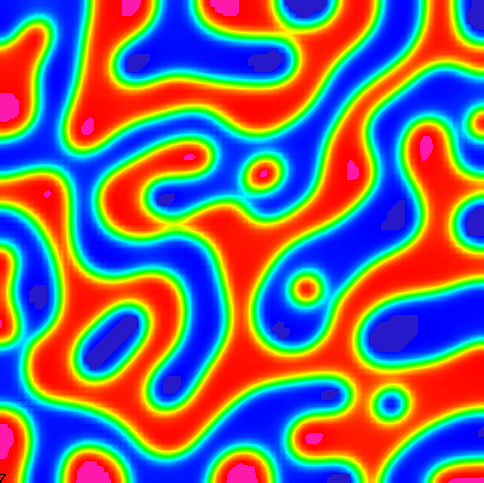
\includegraphics[width=.3\textwidth]{figs/ch100}
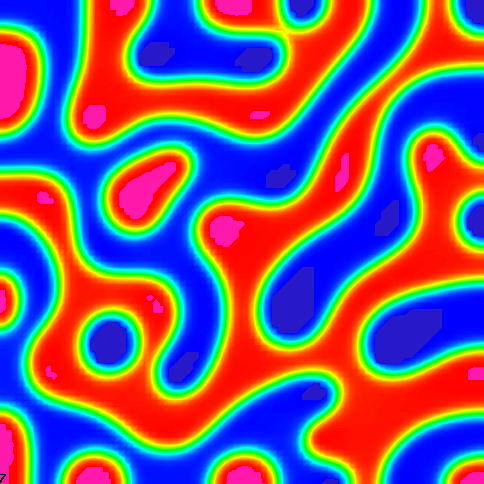
\includegraphics[width=.3\textwidth]{figs/ch200}
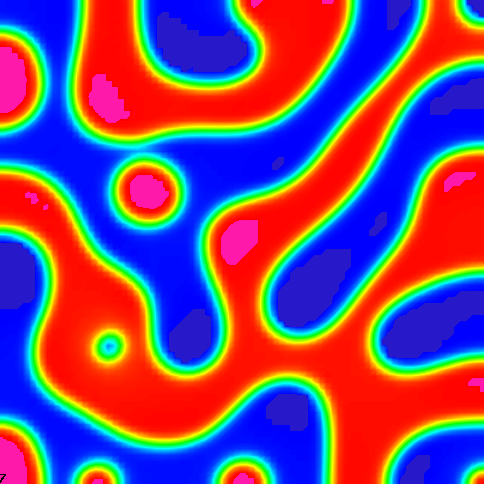
\includegraphics[width=.3\textwidth]{figs/ch500}
\end{center}

}


%%%%%%%%%%%%%%%%%%%%%%%%%%%%%%%%%%%%%%%%%%%%%%%%%%%%%%%%%%%%%%%%%%%%%
\royslide{3D Phase Separation}{

\begin{minipage}[h]{.45\textwidth}
\begin{center}
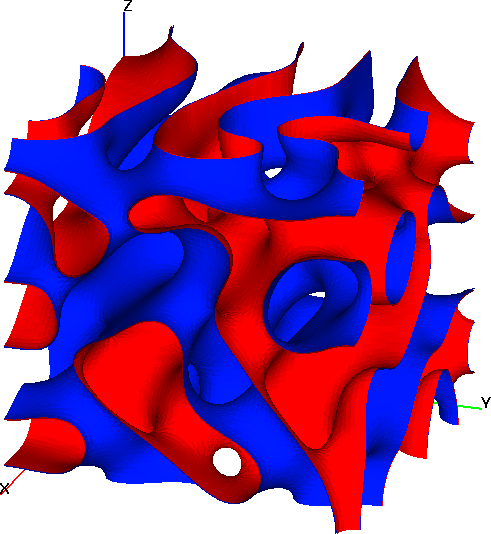
\includegraphics[width=.9\textwidth]{figs/ch-3D}
\end{center}
\end{minipage}
\begin{minipage}[h]{.45\textwidth}
\royitemizebegin
\item Qualitatively similar
\item Topologically very different
\item Much more computationally intensive
\royitemizeend
\end{minipage}

}


%%%%%%%%%%%%%%%%%%%%%%%%%%%%%%%%%%%%%%%%%%%%%%%%%%%%%%%%%%%%%%%%%%%%%
\royslide{Thin Film Patterning}{

\begin{minipage}[h]{.45\textwidth}
\begin{center}
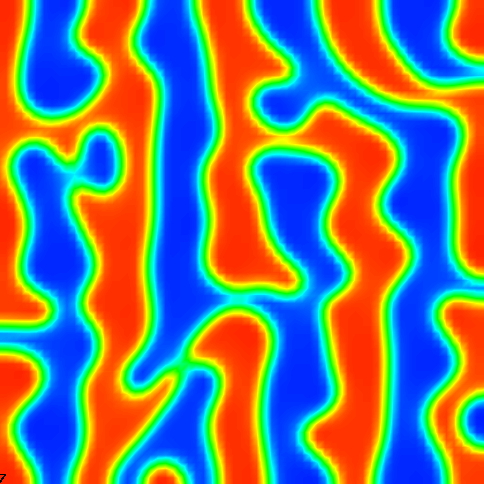
\includegraphics[width=.9\textwidth]{figs/linepattern-example}
\end{center}
\end{minipage}
\begin{minipage}[h]{.45\textwidth}
\royitemizebegin
\item Electrostatic or chemical surface treatment attracts one
material component preferentially
\item A spatially varying bias is added to the configurational free
energy
\royitemizeend
\end{minipage}

}


%%%%%%%%%%%%%%%%%%%%%%%%%%%%%%%%%%%%%%%%%%%%%%%%%%%%%%%%%%%%%%%%%%%%%
\royslide{Effects of Bias Strength}{

Low surface potential energy biases are overwhelmed by random noise

\begin{center}
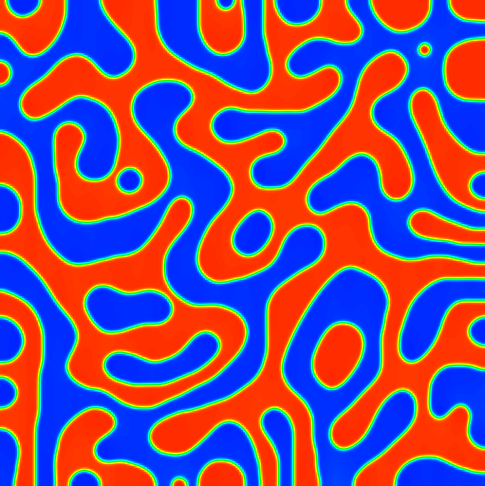
\includegraphics[width=.3\textwidth]{figs/bigpattern-random-0-02}
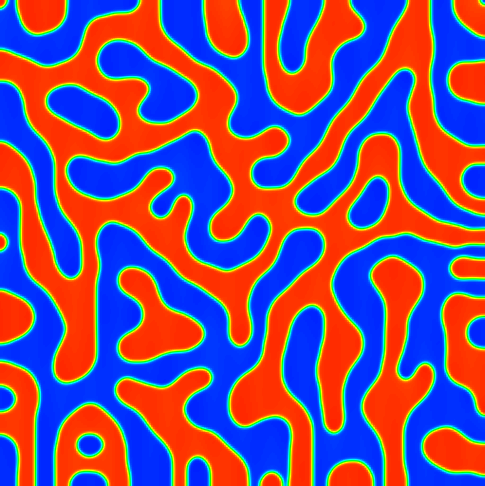
\includegraphics[width=.3\textwidth]{figs/bigpattern-random-0-04}
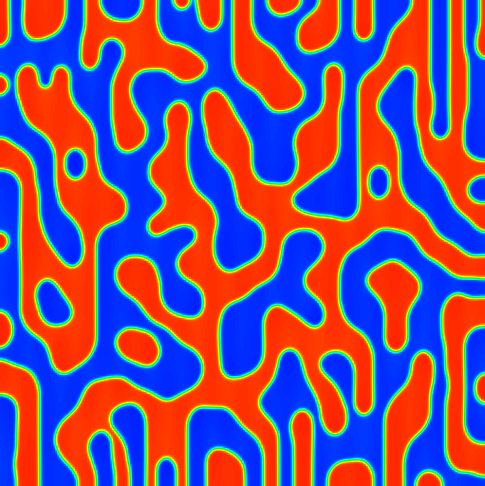
\includegraphics[width=.3\textwidth]{figs/bigpattern-random-0-06}
\end{center}

}


%%%%%%%%%%%%%%%%%%%%%%%%%%%%%%%%%%%%%%%%%%%%%%%%%%%%%%%%%%%%%%%%%%%%%
\royslide{Effects of Bias Strength}{

Higher surface potential energy biases form patterns with decreasing
defect density

\begin{center}
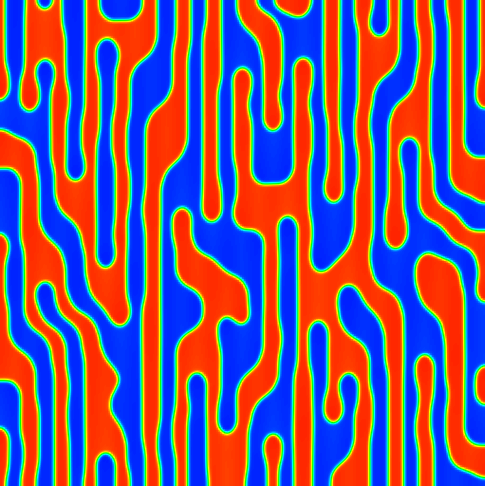
\includegraphics[width=.3\textwidth]{figs/bigpattern-random-0-08}
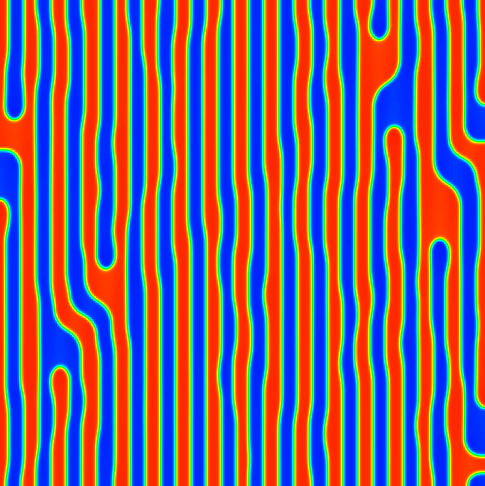
\includegraphics[width=.3\textwidth]{figs/bigpattern-random-0-10}
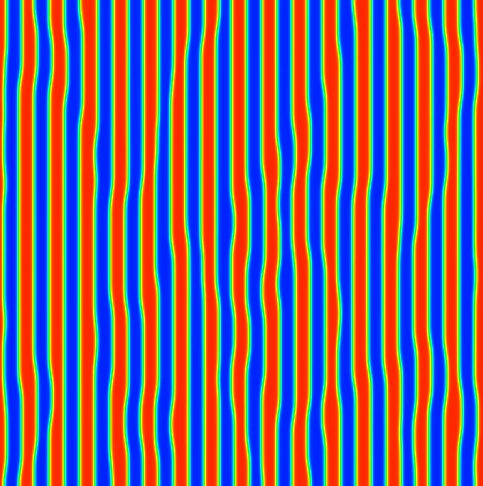
\includegraphics[width=.3\textwidth]{figs/bigpattern-random-0-12}
\end{center}

}
